\section{Neural Low-Degree Filtering}

\label{2605:sec:neural-lofi}

\subsection{Setup and guiding approximation}
We now define Neural LoFi and present its feature-space and kernel interpretations. Its derivation as a surrogate for early gradient-based feature learning is given in App.~\ref{2605:app:GD-neural}. Consider supervised data
\[
    \mathcal D_n=\{(\bm x_\mu,y_\mu)\}_{\mu=1}^n,
    \qquad
    \bm x_\mu\in\mathbb R^d,\quad y_\mu\in\mathbb R,
\]
with scalar labels for simplicity (The extension to vector-valued outputs is discussed in App.~\ref{2605:app:vector-labels}).  We assume throughout this section that the labels are centered, and write
\(\widehat{\mathbb E}_n\) for the empirical average over the training set.  A depth-\(L\) neural network builds a sequence of representations
\begin{equation}
    \bm z_0(\bm x)=\bm x,
    \qquad
    \bm h_\ell(\bm x)
    =
    \bm W_\ell \bm z_{\ell-1}(\bm x),
    \qquad
    \bm z_\ell(\bm x) \in \mathbb{R}^{p_\ell}
    =
    \sigma(\bm h_\ell(\bm x)),
    \qquad
    \ell=1,\dots,L,
    \label{2605:eq:standard-network}
\end{equation}
for sequence of widths $p_1,\cdots, p_L$. For structured architectures, such as convolutional networks, the same notation should be read locally: \({\bm z}_{\ell-1}(\bm x)\) is replaced by the local patch or feature vector seen by a filter, and the corresponding estimator is averaged over spatial locations.
The model's output is then defined by a readout applied to the final layer 
\begin{equation}
    \hat f(x)= \langle \ba_L,\bz_L(x)\rangle.
\end{equation}
Fix a layer \(\ell\), and consider the preactivation
$
    h_{\ell,i}(\bm x)
    =
    \langle \bm w_{\ell,i},\bz_{\ell-1}(\bm x)\rangle 
$. We show  in Appendix \ref{2605:app:GD-neural}, that under a layer-wise vanishing initialization scheme $a_{L} \ll W_{L-1} \ll \cdots W_1$, the training of different neurons in a layer, can be described up to leading approximation through a linear dynamics consisting of two terms: $i)$ a constant drift along a mean direction given by $\hat{\bm u}^\ell \in \mathbb{R}^{p_{\ell}}$
 and $ii)$, a linear projection along the matrix $\widehat{\bm C}^{(\ell)}  \in \mathbb{R}^{p_{\ell} \times p_{\ell}}$, with $\hat{\bm u}^\ell,  \widehat{\bm C}^{(\ell)}$ defined by:
 \begin{equation}\label{2605:eq:lofi-main-operator}
    \hat{\bm u}^\ell \coloneqq \frac{1}{n}\sum_{\mu=1}^n y_{\mu} \bz_{\ell-1}(\bx_\mu) , \quad 
    \widehat{\bm C}^{(\ell)}
    :=
    \frac1n
    \sum_{\mu=1}^n
    y_\mu\,
    \bz_{\ell-1}(\bm x_\mu)
    {\bz}_{\ell-1}(\bm x_\mu)^\top .
\end{equation}

This result is formalized below, which is a consequence of Taylor's theorem and the fact that under a layer-wise vanishing scaling of initializations, interactions between neurons within the same layer and between the present layer and the subsequent, untrained layers, are suppressed: 
\begin{proposition}[Informal]\label{2605:thm:layerwise-GD}
Suppose that  $\hat f(x)$ is trained through layer-wise gradient descent with initialization scale  $a_{L} \ll W_{L-1} \ll \cdots W_1$. Then, for any $\eta>0$, and layer $\ell$, any fixed neuron $w_{\ell,i}$ for $i \in p_{\ell}$, satisfies for small enough time:

\begin{equation}\label{2605:eq:thm1approxmain}
\bw_{\ell,i}(t+1) - \bw_{\ell,i}(t)
\approx \eta\,c_0 \hat{\bu}_\ell
+ \eta\,c_1\widehat{C}^{(\ell)}\,\bw_{\ell,i}(t)+O(\norm{\bw_{\ell,i}(0)}^2),
\end{equation}
for some constants $c_0,c_1>0$.
\end{proposition}

The first term in Eq. \ref{2605:eq:thm1approxmain} is the linear correlation between the current representation and the label. It can be removed by centering, by fitting the best linear predictor in the current representation, or simply interpreted as the degree-one component of the dynamics. The second term, however, is the first genuinely multiple feature-learning component. Let $\widehat{C}^{(\ell)}=\hat{V}\Lambda\hat{V}^\top$ denote the eigendecomposition. For small step-size, the linear term $c_1\widehat{C}^{(\ell)}\,\bw_{\ell,i}(t)$ yields the per-neuron approximation $\bw_{\ell,i}(t)\approx \exp(c_1 \widehat{\bm C}^{(\ell)} t)\,\bw_{\ell,i}(0)$. Stacking the $p_\ell$ neuron weights into the row matrix $W_\ell(t)\in\mathbb{R}^{p_\ell\times p_{\ell-1}}$ with $i$-th row $\bw_{\ell,i}(t)^\top$, the dynamics splits into two interpretable pieces:
\begin{equation}\label{2605:eq:lofi-decomp}
    W_\ell(t)
    \;\approx\;
    W_\ell(0)\,\exp\!\bigl(c_1\,\widehat{\bm C}^{(\ell)}\,t\bigr)
    \;=\;
    \underbrace{W_\ell(0)\,\hat{\bm V}}_{\text{random transformation}} \times \qquad \underbrace{\exp(c_1\,\Lambda\,t)\,\hat{\bm V}^{\!\top}}_{\text{spectral filter}\,\to\,\text{top-eigenvector projection}}\,.
\end{equation}
The second part depends only on $\widehat{\bm C}^{(\ell)}$: it projects onto the eigen-basis of $\widehat{\bm C}^{(\ell)}$ and reweighs each direction by $\exp(c_1\lambda_r^{(\ell)} t)$, exponentially amplifying directions with the largest eigenvalues, so an early-stopped power iteration will approximate hard projection onto the top-$k$ eigenvectors as $t$ grows. The first part $W_\ell(0)\,\hat{\bm V}$ is $t-$independent: it is a fixed random linear transformation of those eigenvectors, inherited from the i.i.d.\ initialization of the neuron weights. 
The post-training feature map $\sigma\bigl(W_\ell(t)\,\bz_{\ell-1}(\bm x)\bigr)$ at each layer is therefore, to leading order, the composition of (i)~a spectral filter that selects the leading eigen-directions of $\widehat{\bm C}^{(\ell)}$ and (ii)~a random per-neuron mixing of those directions: small-initialization training acts, to leading order, as a {\it spectral filtering} of the  representation. \looseness=-1


While the exponential weighting in Equation \ref{2605:eq:lofi-decomp} holds under vanishing initialization and small time-scales, we expect, in general, the network to maintain a preference towards features corresponding to larger eigenvalues for other training regimes. We discuss how weighting regimes arise under different training settings for two-layer networks in App. \ref{2605:app:two-layer}. The simplest choice of such weights is top-$k$ selection: $w(\lambda_r^{(\ell)})=1$ for $r\leq k$ for some $k$, and $0$ otherwise, which we use in Alg.\ref{2605:alg:neural-lofi}. 

Unlike the general gradient descent dynamics involving complex interactions across layers and neurons, the regime identified by Proposition \ref{2605:thm:layerwise-GD} is {\it sequential} across layers and {\it decoupled} across neurons.  We call this the  {\it Neural LoFi regime} and put forward the following hypothesis:
\begin{center}{\it
    The \textbf{Neural LoFi regime} described by Proposition \ref{2605:thm:layerwise-GD} provides a tractable surrogate towards understanding hierarchical learning in deep neural networks.}
\end{center}



\subsection{The Neural Low-Degree Filtering algorithm}
The decomposition in Eq.~\eqref{2605:eq:lofi-decomp} directly motivates the two operations of Neural LoFi (Algorithm~\ref{2605:alg:neural-lofi}), which replace the implicit dynamics of the Neural LoFi regime (Proposition~\ref{2605:thm:layerwise-GD}) with two concrete, decoupled steps per layer: First, a \emph{filter} step projects the current representation onto the leading eigen-directions of the label-weighted moment operator $\widehat{\bm C}^{(\ell)}$, making the spectral filter explicit as $\widehat{\bm V}_\ell$. Second, a \emph{lift} step applies a nonlinear random feature map $\bm R_\ell$ that emulates the per-neuron randomness of the left factor $W_\ell(0)\hat{\bm V}$ in Eq.~\eqref{2605:eq:lofi-decomp}, producing the next representation.
\begin{algorithm}[t]
\caption{Neural Low-Degree Filtering}
\label{2605:alg:neural-lofi}
\begin{algorithmic}[1]
\Require Dataset $\{(\bm x_\mu,y_\mu)\}_{\mu=1}^n$, depth $L$, ranks $\{k_\ell\}_{\ell=1}^L$, widths $\{p_\ell\}_{\ell=1}^L$
\State Initialize $\bm z_0(\bm x)\gets \bm x$ and $p_0 = d$.
\For{$\ell=1,\dots,L$}
    \State $\hat{\bm u}^\ell  \leftarrow \sfrac{1}{n}\sum_{\mu=1}^n y_{\mu} \bz_{\ell-1}(\bx_\mu)$, $\hat{\bm v}^\ell_0 \leftarrow \hat{\bm u}^\ell / \|\hat{\bm u}^\ell\|$
    \Comment{Estimate linear component, normalize}
 %   \State{} % \sfrac{\hat{\bm u}^\ell}{\norm{\hat{\bm u}^\ell}}$ 
    \State Form the label-weighted moment operator:

\[
        \widehat{\bm C}^{(\ell)}
        \gets
        \frac1n
        \sum_{\mu=1}^n
        y_\mu\,
      \bz_{\ell-1}(\bm x_\mu)
        \bz_{\ell-1}(\bm x_\mu)^\top \in \mathbb{R}^{p_{\ell-1} \times p_{\ell - 1}}.
\]

    \State{$
        \widehat{\bm V}_\ell
        =
        [\hat{\bm v}^\ell_0 , \hat{\bm v}^{(\ell)}_1,\dots,\hat{\bm v}^{(\ell)}_{k_\ell}] 
        \in \mathbb{R}^{p_{\ell-1} \times k_\ell}
    $, with ordered \(k_\ell\) eigenvectors by decreasing \(|\hat\lambda|\).}
    \State{$
        \bm g_\ell(\bm x)
        \gets
        \widehat{\bm V}_\ell^\top
        \bz_{\ell-1}(\bm x)
        \in\mathbb R^{k_\ell}.
    $} 
    \Comment{Project onto the learned feature subspace}
    \State{$
        \bm z_\ell(\bm x)
        \gets
        \sfrac{1}{\sqrt{p_\ell}} \sigma(\bm R_\ell \bm g_\ell(\bm x)),
        \,
        \bm R_\ell\in\mathbb R^{p_\ell\times k_\ell}.
    $}
    \Comment{Lift by nonlinear random feature map}
\EndFor
\State{Fit a final linear or logistic readout $\bm a$ on $\bm z_L(\bm x)$.}
\State \Return Final predictor $\hat f(\bm x)=\langle \bm a,\bm z_L(\bm x)\rangle$
\end{algorithmic}
\end{algorithm}

The matrix \(\widehat{\bm V}_\ell\) defines the \emph{learned feature projection} at layer \(\ell\). The projections
\begin{equation}
    \bm g_\ell(\bm x)
    =
    \widehat{\bm V}_\ell^\top
    \bz_{\ell-1}(\bm x)
    \label{2605:eq:learned-feature-projection}
\end{equation}
are the features selected by low-degree filtering. The random nonlinear lift \(\sigma(\bm R_\ell \bm g_\ell)\) then re-expands these selected coordinates into a richer representation, so that the next layer can search for new low-degree correlations in the transformed feature space.
The projection step can be interpreted as a {\it weighted principal component analysis}: The linear component $\hat{\bm u}^\ell$ gives the direction in the feature space $\bz_{\ell-1}(\bm x)$ maximizing the linear correlation with $y$, and the top eigenvectors of $ \widehat{\bm C}^{(\ell)}$ extract the most relevant directions\footnote{In some experiments, we did not even kept the linear component, as the second-order components are numerous and seem to suffice for extracting the most relevant features.} in feature space $\bz_{\ell-1}(\bm x)$ weighted by their $2^{nd}$-order correlation with $y$. 




\begin{figure}
    \centering
    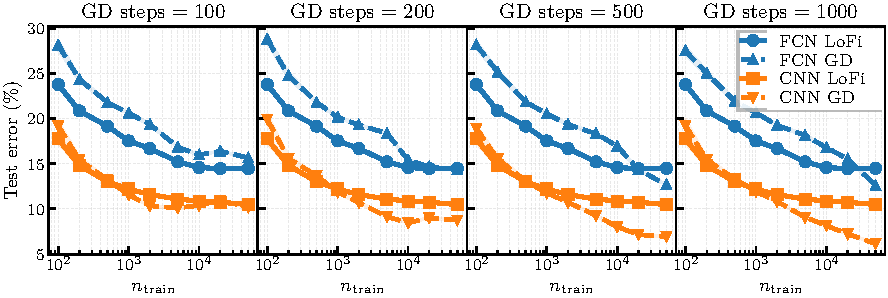
\includegraphics[width=\linewidth]{figs/error_line}
    \caption{\textbf{Neural LoFi versus gradient descent/backpropagation (GD).}
Test error on binary CIFAR-10 \cite{krizhevsky2009learning} (animals vs. vehicles) for fully connected networks (FCN) and convolutional networks (CNN). We compare Neural LoFi with networks trained by gradient descent/backpropagation, shown for different numbers of training steps. In the low-data regime, and at early training times even with more data, Neural LoFi matches or exceeds GD, illustrating that the spectral surrogate captures an efficient supervised feature-extraction mechanism.
}
\label{2605:fig:gd-lofi-comparison}
\end{figure}

Figure~\ref{2605:fig:gd-lofi-comparison} gives a first sanity check for Neural LoFi as a surrogate for gradient-based feature learning. We compare it with backpropagation on the binary CIFAR-10 animal-vs.-vehicle task, for both fully connected and convolutional architectures. The results show that Neural LoFi can match early GD performance, especially in the low-data regime, while remaining a one-pass spectral procedure. We return to these experiments in detail in Section~\ref{2605:sec:real-data}.

\subsection{Function-space and kernel interpretation}
The projection components $[\hat{\bm v}^\ell_0 , \hat{\bm v}^{(\ell)}_1,\dots,\hat{\bm v}^{(\ell)}_{k_\ell}]$ reside in the dual space w.r.t. the features $\bz_{\ell-1}$ and are themselves not directly interpretable and depend on the choice of random projection weights $R_{\ell-1},\cdots, R_1$. However, we show below that the resulting features $\langle\hat{\bm u}^{(\ell)},\bz_{\ell-1}(\bm x)\rangle$ and $\langle \hat{\bm v}^{(\ell)}_j,\bz_{\ell-1}(\bm x)\rangle$, for $j=1,\dots,k_\ell$, admit a clear description in terms of low-degree projections of $y$ onto the RKHS defined by the previous layer. Furthermore, the features converge to deterministic infinite-width limits. Let
\begin{equation}
    K_{\ell-1}(\bm x,\bm x')
    =
    \langle
    \bz_{\ell-1}(\bm x),
    \bz_{\ell-1}(\bm x')
    \rangle
    \label{2605:eq:lofi-current-kernel}
\end{equation}
be the kernel induced by the current representation, and let \(\mathcal H_{\ell-1}\) be its Reproducing Kernel Hilbert Space (RKHS \cite{steinwart2008support,scholkopf2002learning}). Through an analogue of the classical representer theorem (Lemma \ref{2605:lem:representer-lofi}), we show that for any $j \in k_{\ell}$, the features
$
    \varphi_{j}(\bm x)
    \coloneqq
    \langle \hat{\bm v}^{(\ell)}_j, \bz_{\ell-1}(\bm x)\rangle$, lie in the subspace spanned by $\{K_{\ell-1}(\bm x_{\mu},\cdot)\}_{\mu=1}^n$, and satisfy the equivalence of norms given by \(\|\varphi_{j}(\bm x)\|_{\mathcal H_{\ell-1}}=\|\hat{\bm v}^{(\ell)}_j\|_2\). 
Since $\hat{\bm v}^{(\ell)}_1$ maximizes $\bv^\top\widehat{\bm C}^{(\ell)}\bv$ subject to the $\|\bm v\|_2=1$, we obtain the equivalent criterion:
\begin{equation}
\hat{\bm v}^{(\ell)}_1
    \in
    \argmax_{\|\bm v\|_2=1}
    \left|
    \frac1n
    \sum_{\mu=1}^n
    y_\mu
    \langle \bm v,\bz_{\ell-1}(\bm x_\mu)\rangle^2
    \right|
\rightarrow
    \varphi_1^{(\ell)}
    \in
    \argmax_{\|\varphi\|_{\mathcal H_{\ell-1}}=1}
    \left|
    \frac1n
    \sum_{\mu=1}^n
    y_\mu\,\varphi(\bm x_\mu)^2
    \right|.
    \label{2605:eq:lofi-rkhs-variational}
\end{equation}
Maximizing this correlation with the label, together with the norm constraint in feature space, leads to the fundamental conclusion:

\emph{
Neural LoFi searches for features that are {\bf simple} in the geometry induced by the previous layer, but {\bf predictive} through their low-degree correlation with the task.}

This is the sense in which the method is a low-degree filter.  We show in App.\ref{2605:app:kernel-nlofi}, how this can  be turned into a practical kernel version of our approach. This is formalized through the following result, furthermore showing that they converge to the eigenfunctions of the limiting infinite-width kernel as the layer width grows:
\begin{theorem}[Variational characterization and infinite-width convergence]
\label{2605:thm:variational-rkhs}
Let $\hat{\bm v}^\ell_0$ denote the linear component and $[\hat{\bm v}^{(\ell)}_1,\dots,\hat{\bm v}^{(\ell)}_{k_\ell}]$ the ordered eigenvectors from Algorithm~\ref{2605:alg:neural-lofi}. 
Define the linear feature
\[
    \psi^\ell(\bm x) \coloneqq \langle \hat{\bm v}^\ell_0,\, \bz_{\ell-1}(\bm x)\rangle,
\]
and the second-order features $\varphi_j(\bm x) \coloneqq \langle \hat{\bm v}^{(\ell)}_j,\bz_{\ell-1}(\bm x)\rangle$ for $j=1,\dots,k_\ell$. Then:
\begin{enumerate}[label=(\roman*),noitemsep,leftmargin=1em,wide=0pt]
    \item \textbf{Linear feature.} $\psi^\ell$ is the unit-norm maximizer of the empirical first-order correlation with $y$:
    \begin{equation}
        \psi^\ell \;=\; \argmax_{\psi:\,\|\psi\|_{\mathcal H_{\ell-1}}=1}
        \left|\,\widehat{\mathbb E}_n\bigl[y\,\psi(\bm x)\bigr]\,\right|.
        \label{2605:eq:prop-linear-var}
    \end{equation}
    \item \textbf{Second-order features.} For each $k=1,\dots,k_\ell$, $\varphi_k$ is the unit-norm maximizer of the empirical second-order correlation, successively orthogonalized to the previously selected features:
    \begin{equation}
        \varphi_k \;=\; \argmax_{\substack{\varphi:\,\|\varphi\|_{\mathcal H_{\ell-1}}=1\\ \varphi\perp\varphi_1,\dots,\varphi_{k-1}}}
        \left|\,\widehat{\mathbb E}_n\bigl[y\,\varphi(\bm x)^2\bigr]\,\right|.
        \label{2605:eq:prop-quadratic-var}
    \end{equation}
    \item \textbf{Infinite-width convergence.} Let $K^{\infty}_{\ell-1}$ denote the infinite-width limiting kernel obtained as the layer width $p_{\ell-1}\to\infty$, and let $\{\phi^{\infty}_k\}_{k\geq 1}$ be its eigenfunctions ordered by decreasing eigenvalue magnitude with the selected limiting eigenvalues separated from the rest of the spectrum. Then, for any  pseudo-lipschitz (of finite order) $\sigma(\cdot)$, and any fixed $k$, as $p_{\ell-1}\to\infty$,
    \[
        \varphi_k \;\xrightarrow{\;\;\;}\; \phi^{\infty}_k,
    \]
    where convergence is in $L^2$ under the data distribution, and $\phi^{\infty}_1,\cdots, \phi^{\infty}_k$ satisfy the corresponding limiting {\it deterministic} variational criteria.
\end{enumerate}
\end{theorem}

The above characterization in feature space translates to an explicit recursion over the kernels defined by each layer, once the selected features
$
    \varphi_1^{(\ell)},\dots,\varphi_{k_\ell}^{(\ell)}
$ are obtained, define
$
    \bm g_\ell(\bm x)
    =
    \big(
    \varphi_1^{(\ell)}(\bm x),\dots,\varphi_{k_\ell}^{(\ell)}(\bm x)
    \big).
$
If the next layer is a random nonlinear lift, then the induced kernel is
\begin{equation}
    K_\ell(\bm x,\bm x')
    =
    \mathbb E_{\bm r}
    \left[
    \sigma(\bm r^\top \bm g_\ell(\bm x))
    \sigma(\bm r^\top \bm g_\ell(\bm x'))
    \right].
    \label{2605:eq:lofi-kernel-recursion}
\end{equation}

This recursion is the kernel-level form of feature learning. Unlike a {\it fixed} kernel method, with a single geometry before seeing the labels, Neural LoFi constructs a sequence of task-adaptive kernels
$K_0 \longrightarrow K_1 \longrightarrow \cdots \longrightarrow K_L$,
where each transition is supervised: the next kernel is built from the low-complexity features in \(\mathcal H_{\ell-1}\) whose squared activations are most correlated with the label.  Neural LoFi thus turns deep learning into an explicit procedure for adaptive kernel construction. %In this sense, it answers the {\it quest for adaptivity} of kernel methods: depth is not merely a fixed richer kernel, but a mechanism for changing the kernel geometry layer by layer according to the task.
